\documentclass[12pt]{article}
\usepackage[margin=2.5cm]{geometry}
\usepackage{enumerate}
\usepackage{amsfonts}
\usepackage{amsmath}
\usepackage{fancyhdr}
\usepackage{amsmath}
\usepackage{amssymb}
\usepackage{amsthm}
\usepackage{mdframed}
\usepackage{graphicx}
\usepackage{subcaption}
\usepackage{adjustbox}
\usepackage{listings}
\usepackage{xcolor}
\usepackage{soul}
\usepackage{booktabs}
\usepackage[utf]{kotex}
\usepackage{hyperref}

\definecolor{codegreen}{rgb}{0,0.6,0}
\definecolor{codegray}{rgb}{0.5,0.5,0.5}
\definecolor{codepurple}{rgb}{0.58,0,0.82}
\definecolor{backcolour}{rgb}{0.95,0.95,0.92}

\lstdefinestyle{mystyle}{
    backgroundcolor=\color{backcolour},
    commentstyle=\color{codegreen},
    keywordstyle=\color{magenta},
    numberstyle=\tiny\color{codegray},
    stringstyle=\color{codepurple},
    basicstyle=\ttfamily\footnotesize,
    breakatwhitespace=false,
    breaklines=true,
    captionpos=b,
    keepspaces=true,
    numbers=left,
    numbersep=5pt,
    showspaces=false,
    showstringspaces=false,
    showtabs=false,
    tabsize=1
}

\lstset{style=mystyle}

\pagestyle{fancy}
\renewcommand{\headrulewidth}{0.4pt}
\lhead{CSC 373}
\rhead{Worksheet 6 Solution}

\begin{document}
\title{CSC373 Worksheet 6 Solution}
\maketitle

\bigskip

\begin{enumerate}[1.]
    \item

    \bigskip

    \underline{\textbf{Notes:}}

    \bigskip

    \begin{itemize}
        \item \textbf{Linear Programming}
        \begin{itemize}
            \item Is a method to achieve the best outcome (such as maximum profit or lowest cost) in a mathematical model
            whose requirements are represented by linear relationships. $^{[1]}$
            \item Is named to make it sound cool for government funding
            \begin{itemize}
                \item Like dynamic programming
            \end{itemize}
            \item Applications

            \begin{itemize}
                \item Microeconomics (maximize profits, minimize costs)
                \item Company management
            \end{itemize}
        \end{itemize}

        \item \textbf{Standard Form}

        \begin{itemize}
            \item Is a form of linear programming
            \item Are about \ul{maximizing}, not minimizing $^{[2]}$
            \item All variables involved are restricted to be non-negative $^{[3]}$
            \item All constraints are equalities, with constant, non-negative right-hand $^{[3]}$
            sides
        \end{itemize}

        \bigskip

        \underline{\textbf{Example:}}

        \bigskip

        \begin{center}
        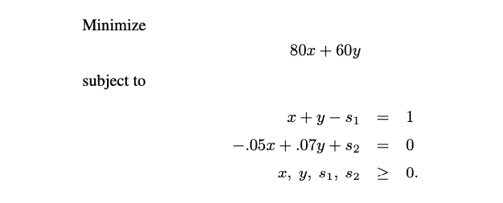
\includegraphics[width=0.8\linewidth]{images/worksheet_6_solution_1.png}
        \end{center}

        \item \textbf{Converting Linear Programming to Standard Form}

        \begin{enumerate}[1)]
            \item Mutliply inequality by -1 to get non-negative RHS $^{[3]}$
            \item Convert inequalities to equalities by adding or subtracting
            non-negative slack variables $^{[3]}$
            \item Resolve unrestrictive variables by writing the variable as
            the difference of two new non-negative variables $^{[3]}$
        \end{enumerate}

        \bigskip

        \underline{\textbf{Example:}}

        \begin{center}
        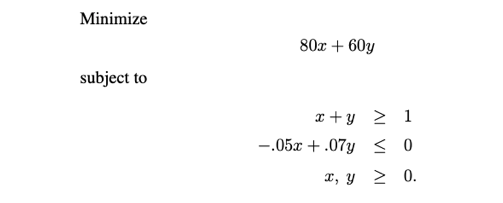
\includegraphics[width=0.8\linewidth]{images/worksheet_6_solution_2.png}
        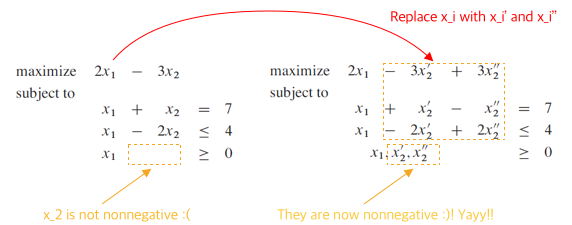
\includegraphics[width=0.8\linewidth]{images/worksheet_6_solution_3.png}
        \end{center}
    \end{itemize}

    \bigskip

    \underline{\textbf{References:}}

    \bigskip

    \begin{enumerate}[1)]
        \item Wikipedia, Linear Programming, \href{https://en.wikipedia.org/wiki/Linear_programming}{link}
        \item Instituto de Mathematicas, Standard form for Linear Programs, \href{https://www.matem.unam.mx/~omar/math340/std-form.html}{link}
        \item University of Notre Dame, Converting an LP to standard form, \href{https://www3.nd.edu/~dgalvin1/30210/30210_F07/presentations/converting.pdf}{link}
    \end{enumerate}
\end{enumerate}

\end{document}